\chapter{Pair localization transition}\label{ch:pair-localization-transition}

In this chapter, we address the question: Does the model defined in Eq.~\ref{eq:heisenberg-hamiltonian} exhibit a localization crossover for sufficiently strong disorder? To this end, we compute the level-spacing ratio, Thouless parameter and half-chain entropy to detect the crossover into a localized regime and use the shot-to-shot variance of the half-chain entropy to perform finite size scaling of the crossover's location. Indeed, all indicators confirm the presence of a localized regime. Remarkably, the location of the crossover in this system appears to be significantly more stable than in systems with random on-site potentials. Additionally, we employ the strong disorder/real-space renormalization group (RSRG) approach to show that the quasi-conserved quantities are given by strongly interaction pairs of spins, which demonstrate numerically by computing participation ratios between the approximated and exact eigenbases.

In summary, we find that for sufficiently strong disorder the complicated many-body system given by Eq.~\ref{eq:heisenberg-hamiltonian} can be well approximated by an integrable model of pairs:
\begin{align}\label{eq:pair-model}
	H_{pairs} =& \sum_{\langle i,j\rangle} \left(S_x^{(i)}S_x^{(j)} + S_y^{(i)}S_y^{(j)} + \Delta S_z^{(i)}S_z^{(j)}\right) \notag\\
	+ &\sum_{\substack{\langle i,j\rangle\\\langle i',j'\rangle}} \frac{\Delta}{4}(J_{i,i'}+J_{i,j'}+J_{j,i'}+J_{j,j'})\left(S_z^{(i)}+S_z^{(j)}\right)\left(S_z^{(i')}+S_z^{(j')}\right)
\end{align}
Here $\sum_{\langle i,j\rangle}$ denotes a sum over specific pairs of spins in the RSRG sense. These pairs are found iteratively: One defines the two spins linked by the strongest coupling in the system to be a pair, removes them and then continues with the remaining spins until every spin is paired up. This model of pairs is validated experimentally in Chapter~\ref{ch:experimental-pairs} and proves to give very accurate results.

\newpage
\pdfbookmark[2]{Publication}{pairlocalization-paper}
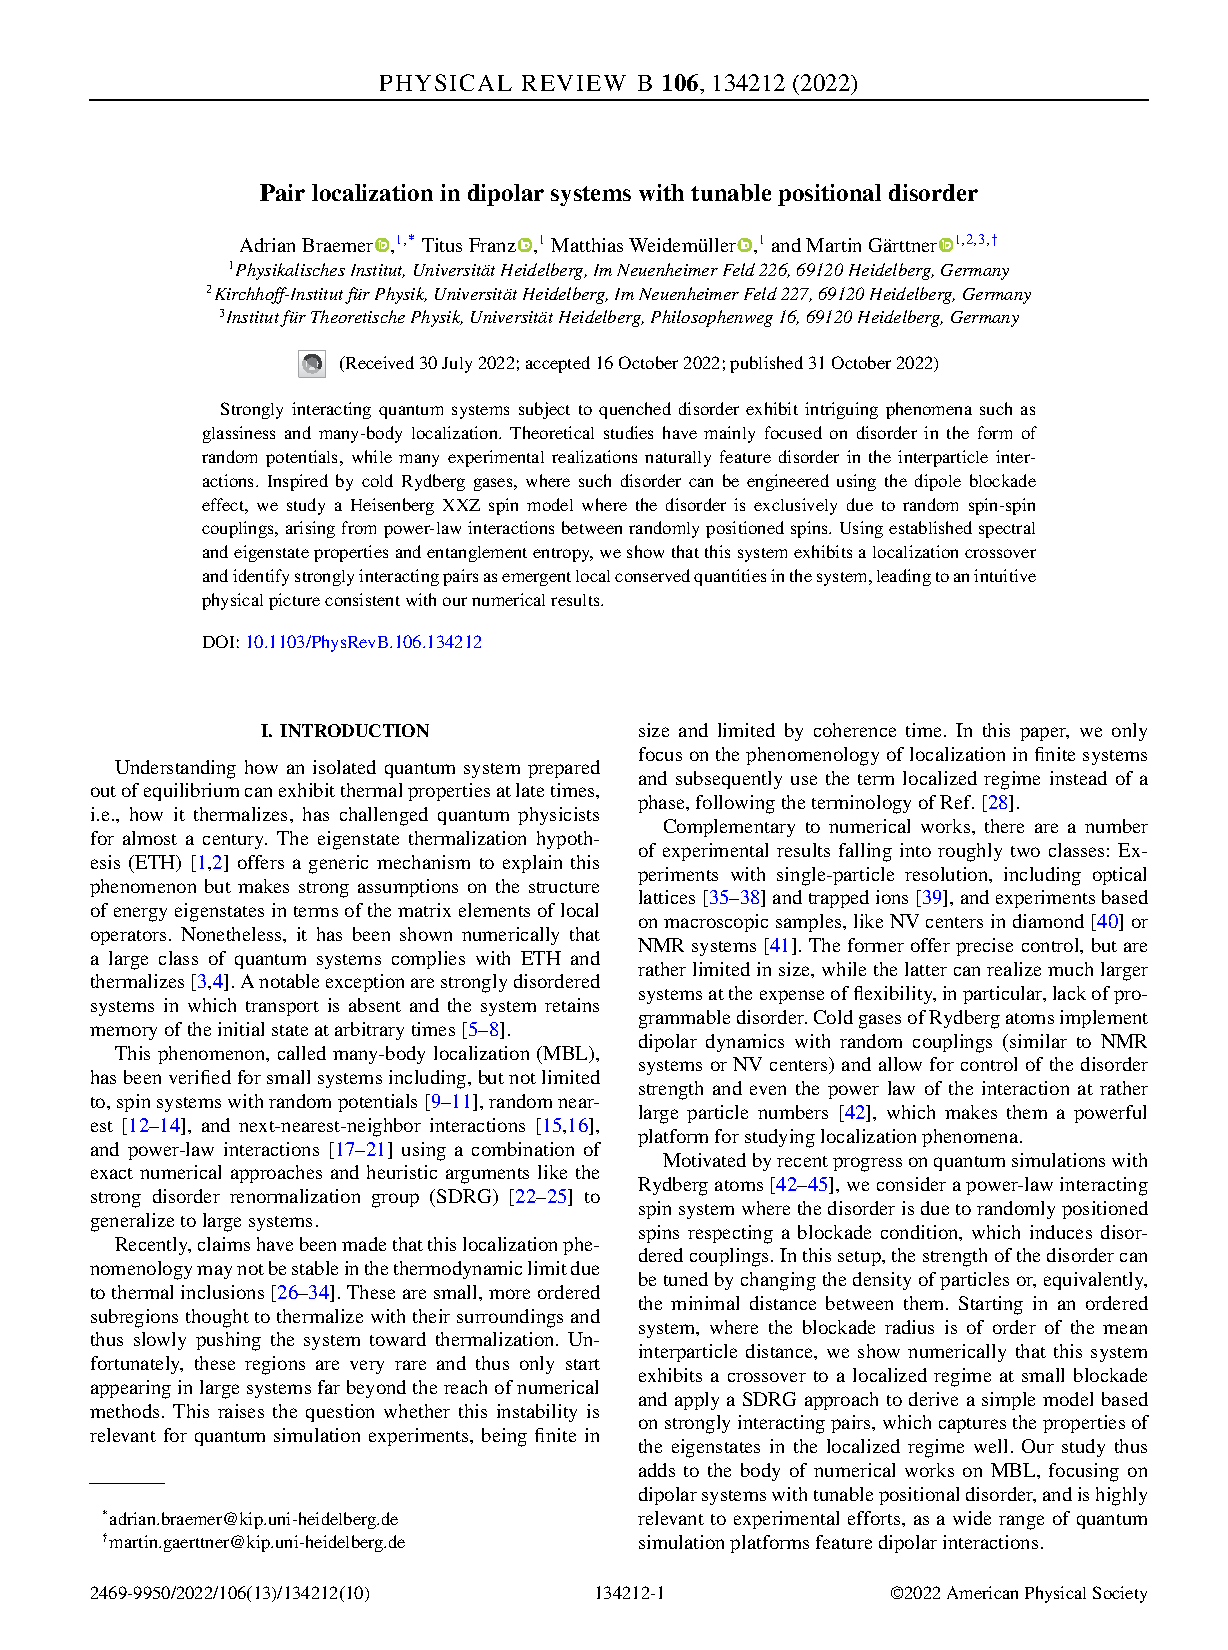
\includepdf[pages=-]{pub-Braemer2022-Pairlocalization}

\chapter{Efficient time evolution of pair localized systems}\label{ch:cTWA-paper}

After having found an analytical approximation applicable at strong disorder in the preceding chapter, here we show how to utilize this knowledge to achieve an efficient numerical computation of the dynamics. The key idea is to employ the cluster truncated Wigner approximation~\cite{wurtzClusterTruncatedWigner2018}, which is a semiclassical simulation method that solves the dynamics of only small clusters of spins exactly and treats interactions among clusters on a mean-field level. By using the pairing procedure of Chapter~\ref{ch:pair-localization-transition} to define the clusters, we find that our method is highly accurate not only at strong disorder and short-range interactions but also in regimes of comparatively weak disorder and long-range interactions. 
Thus, our method represents a numerically efficient scheme to compute arbitrary dynamical quantities in these kinds of spatially disordered spin systems.

% In addition, we generalize the cluster truncated Wigner approximation slightly to use a discrete phase-space sampling, which offers a minor boost in performance compared to continuous sampling and simplifies the implementation slightly since clusters of single spins no longer represent a special case. 
%TODO also mention the sampling? Not really important in the context of this work though
\newpage
\pdfbookmark[2]{Publication}{cTWA-paper}
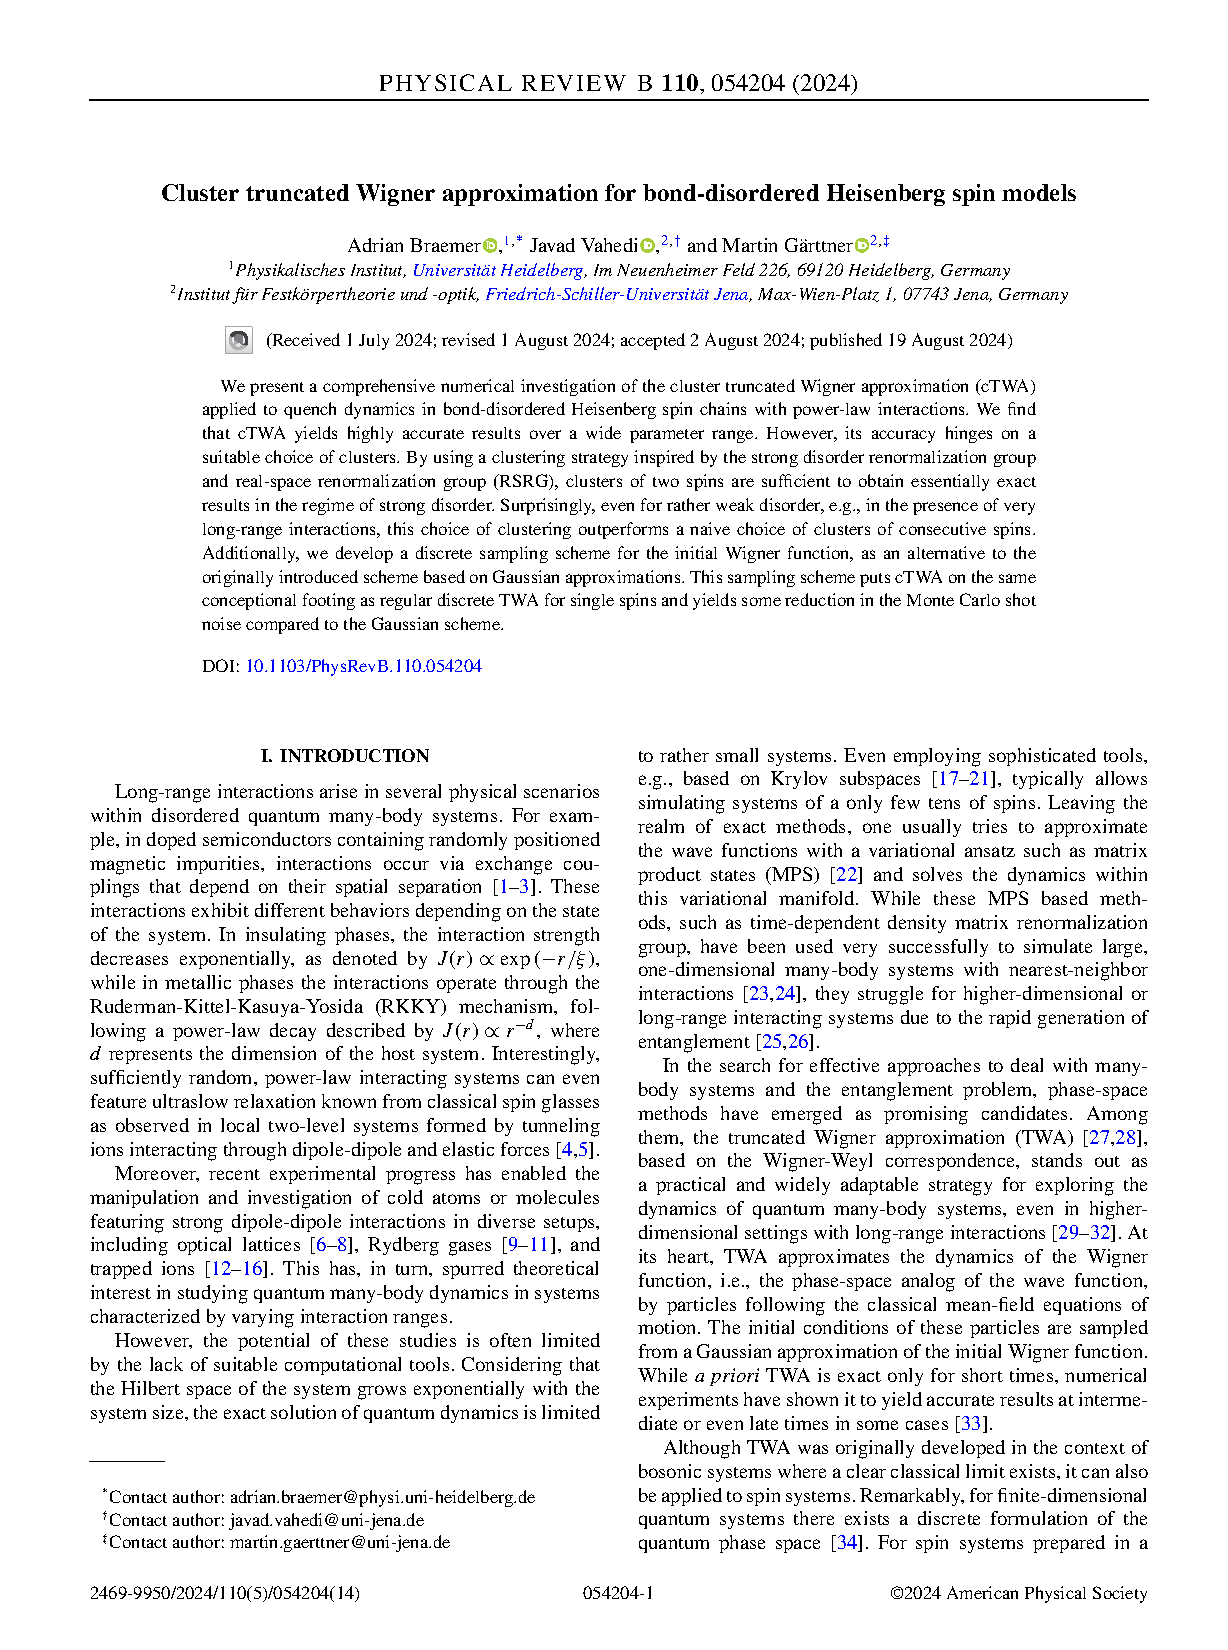
\includepdf[pages=-]{pub-Braemer2024-cTWA}